\section{Completed text experiments and follow-up diagnostics}
\label{sec:newresults}
This revision incorporates the completed passage, HelpSteer, semantic-MMD,
calibrated-kernel, continuation, and distribution-only records available on
November 22, 2026. The preceding sections preserve the original methods;
this section reports achieved budgets and outcomes, including unsuccessful
trials. No new GPU experiment was run to prepare this revision.

\subsection{Shared conventions and scope of comparison}
All text actors start from the pinned Qwen2.5-3B-Instruct checkpoint,
revision \texttt{aa8e72537993} (full hash in the source records), with a fresh
attention-LoRA adapter (rank 16, alpha 32, dropout zero), except the
explicit energy continuation below. They do not start from the numeric
SFT adapter. On-policy passage-level REINFORCE uses AdamW, actor learning
rate $5\times10^{-6}$, weight decay 0.01, and clipping at one.
There is no trained value critic, PPO clipping, replayed multi-epoch PPO
update, or GRPO clipped likelihood-ratio objective. Leave-one-out
baselines alone do not turn the implementation into GRPO.

Table~\ref{tab:text-inventory-new} records actual updates rather than
planned ceilings. Most text studies use two H200s and stop at a time
budget. Different targets, prompt sets, answer counts, caps, quality
scorers, and schedules preclude treating every row as a controlled
algorithm comparison. Absolute word KL, Gaussian discrepancy, energy
distance, and reward scores across protocols are not a common scale.
Baselines and final policies within each comparison use matched decoding
settings and evaluation seeds. All reported logarithms use natural units.
No generated policy answer was newly rated by humans for these studies.
\begin{table}[htbp]
\centering\footnotesize
\caption{Achieved text-policy budgets, not configured update ceilings. Minutes are each comparison record's measured process time, not scheduler allocation limits. The energy continuation adds 147 updates to 53 existing updates; its cumulative total is 200.}\label{tab:text-inventory-new}
\begin{tabular}{@{}lrrrr@{}}
\toprule
Policy trial & H200s & Updates & Training answers & Minutes\\
\midrule
Shakespeare pilot & 1 & 100 & 1,600 & 17.4\\
Shakespeare bigram & 2 & 1,200 & 19,200 & 101.1\\
Shakespeare unigram & 2 & 1,097 & 17,552 & 105.6\\
Subset quality only & 2 & 200 & 3,200 & 29.3\\
Subset word KL 0.1 & 2 & 200 & 3,200 & 27.9\\
Subset word KL 0.5 & 2 & 200 & 3,200 & 28.1\\
Broad word KL & 2 & 86 & 1,376 & 80.0\\
Programming word KL & 2 & 75 & 1,200 & 85.3\\
Gaussian MMD v1 & 2 & 94 & 1,504 & 81.3\\
Calibrated Gaussian & 2 & 50 & 800 & 52.1\\
Calibrated energy & 2 & 53 & 848 & 51.3\\
Energy continuation & 2 & 147 & 2,352 & 119.7\\
Distribution only & 2 & 17 & 1,088 & 77.7\\
\bottomrule
\end{tabular}
\end{table}


\subsection{Shakespeare passage matching: judge repair and completed runs}
An intermediate experiment matches a pooled TinyShakespeare training
corpus while asking for intelligible original dramatic passages. The
initial JSON-output judge audit exposed missing prompt-fulfillment scores
in 22 of 48 passages; it is not a valid quality benchmark. The repaired
frozen Qwen2.5-7B-Instruct judge scores each dimension separately using
the expected digit conditional on the 1--5 rating tokens. Six anchor
passages each outranked shuffled-word and repeated controls on coherence
and off-prompt controls on fulfillment, passing all 18 predefined
comparisons. These perturbation checks support implementation sensitivity,
not human-level reliability or calibration.

For these passage trials, the quality reward is the mean of coherence,
fluency, and prompt-fulfillment scores mapped from 1--5 to 0--1; capped
outputs receive zero quality but retain observed histogram counts. The
objective combines quality with negative target histogram KL at weight
0.1 and initial-policy KL at weight 0.002. The contiguous corpus split,
pinned to \texttt{karpathy/char-rnn} revision \texttt{370cbcd}, is neither
play-disjoint nor demonstrated free of pretraining overlap. The bigram
reference contains 83,454 word-pair types plus UNK; the unigram reference
contains 10,948 word types plus UNK, with total smoothing mass one.
The cap is 256 new tokens; the main runs use 16 global passages per update.

The one-H200 pilot completed 100 updates and 1,600 passages. On its own
four-prompt test (64 passages), bigram KL changed 7.9903 to 7.9935 and
quality 0.7544 to 0.7615. Termination changed 63/64 to 64/64, while all
three raw judge dimensions decreased slightly. This illustrates how
aggregate rewards can be affected by termination rules. Its smaller
prompt set prevents attributing differences from later runs solely to
training duration.

The two-H200 bigram run completed 1,200 updates and 19,200 passages;
the unigram run completed 1,097 updates and 17,552 passages. Both use
the same 16 held-out scenarios, four draws each, and the same instruction
baseline (Table~\ref{tab:passage-new}). Both lower measured word and
word-pair KL and raise the shared judge reward. Bigram-trained quality
improves on 15/16 scenarios, with a recorded exploratory prompt-bootstrap
mean-change interval $[0.0417,0.0836]$. Unigram-trained quality improves
on 14/16, with interval $[0.0067,0.0815]$. Comparing unigram to bigram
quality gives $-0.0155$, interval $[-0.0459,0.0049]$, and eight scenario
wins each; there is no clear quality winner.
\begin{table}[htbp]
\centering\small
\caption{Shakespeare test: 16 held-out scenarios, four passages each. KL is pooled and smoothed; quality is the same frozen judge used in training.}\label{tab:passage-new}
\begin{tabular}{@{}lrrrrr@{}}
\toprule
Policy (updates) & Word KL & Pair KL & $r_Q$ & Words & EOS (\%)\\
\midrule
Instruction base & 3.0598 & 8.0710 & 0.7419 & 96.9 & 100.0\\
Bigram RL (1,200) & 2.7766 & 7.9282 & 0.8029 & 115.5 & 100.0\\
Unigram RL (1,097) & 2.5876 & 7.8699 & 0.7874 & 137.2 & 98.4\\
\bottomrule
\end{tabular}
\end{table}


The bigram model's coherence/fluency/fulfillment scores change from
3.8499/3.9618/4.0913 to 3.9985/4.0354/4.6011. The unigram model reaches
3.9821/4.0285/4.5827. Bigram outputs are 19.2\% longer than baseline;
unigram outputs are 41.6\% longer. Count matching still favors both
trained policies (Table~\ref{tab:passage-counts}), but does not remove
histogram-estimator bias or passage dependence. Out-of-reference word
mass falls from 11.37\% to 9.66\% (bigram) and 7.88\% (unigram).
No source-overlapping 12-word windows were found in the evaluated
passages; this limited diagnostic does not exclude memorization.
These are positive findings under the training judge, without a
quality-only control, equal-compute SFT, new human evaluation, or a
second training seed.
\begin{table}[htbp]
\centering\small
\caption{Post hoc count matching: 200 subsamples without replacement, 6,200 words or 6,136 word pairs per policy (seed 20261119).}\label{tab:passage-counts}
\begin{tabular}{@{}lrr@{}}
\toprule
Policy & Matched word KL & Matched pair KL\\
\midrule
Instruction base & 3.0598 & 8.0710\\
Bigram RL & 2.8589 & 7.8776\\
Unigram RL & 2.7006 & 7.7929\\
\bottomrule
\end{tabular}
\end{table}


\subsection{HelpSteer subset trials and stronger reward selection}
The original protocol in Section~\ref{sec:helpsteer} prepares a larger
533-prompt policy pool. The completed exploratory subset instead uses
128 policy/reference training prompts, eight validation prompts and 16
test prompts. Each of three arms completes 200 updates with 16 answers
per update. Its locally fitted 3B Bradley--Terry scorer is frozen during
actor training. With a 384-token cap, incomplete answers receive zero
quality, and only 53--59\% of final test answers terminate.
Neither quality-only nor either word-KL weight improves both target KL
and quality (Table~\ref{tab:subset-new}). These outcomes supersede the
earlier pending status; they do not establish that a full 600-update
profile was completed.
\begin{table}[htbp]
\centering\small
\caption{Initial short-answer HelpSteer subset: each arm completed 200 updates and 3,200 training answers. Evaluation: 16 prompts, two answers each; cap 384 tokens.}\label{tab:subset-new}
\begin{tabular}{@{}lrrrr@{}}
\toprule
Policy & $\lambda$ & Word KL & $r_Q$ & EOS (\%)\\
\midrule
Instruction base & --- & 2.7988 & 0.3663 & 59.4\\
Quality only & 0.0 & 2.8067 & 0.3293 & 53.1\\
Quality + word KL & 0.1 & 2.8444 & 0.3623 & 59.4\\
Quality + word KL & 0.5 & 2.8801 & 0.3461 & 56.2\\
\bottomrule
\end{tabular}
\end{table}


A subsequent, expanded-input reward-model audit uses a separate profile
with 280 non-tied human preference pairs, rather than the original
216-non-tie validation subset. It compares with a longer-answer baseline (63.93\%) and
a training-majority-direction baseline (56.79\%). The local BT scorer
achieves 67.14\%, but its paired accuracy margin over the length baseline
has interval $[-4.29,11.43]$ percentage points, failing the stronger gate.
The frozen \texttt{Skywork/Skywork-Reward-V2-Qwen3-8B} achieves 78.75\%;
its margin over length has interval $[8.57,21.79]$ points and over
majority $[14.82,28.93]$ points. It passes all six predefined checks,
including length-matched, human-coherence and long-input evidence.
Table~\ref{tab:reward-audit-new} summarizes the main strata.
Long-input accuracies are 75.0\% on 64 pairs (local) and 77.5\% on 60
pairs (Skywork); tokenizer-dependent eligibility means these are not
identical denominators. The audit is scorer-selection validation,
not an independent final test. Public reward-model training overlap
with HelpSteer is unknown.
\begin{table}[htbp]
\centering\footnotesize
\caption{Stronger reward-model selection audit. Main accuracy: 280 non-tied human-preference pairs; length matched: 73; coherence comparisons: 146. All accuracies in percent. Intervals describe validation selection, not an independent benchmark.}\label{tab:reward-audit-new}
\begin{tabular}{@{}lrrrrr@{}}
\toprule
Scorer & Accuracy & 95\% interval & Length & Coherence & Gate\\
\midrule
Local BT 3B & 67.1 & [61.8, 72.5] & 64.4 & 65.4 & Fail\\
Frozen Skywork 8B & 78.8 & [73.9, 83.6] & 71.9 & 78.8 & Pass\\
\bottomrule
\end{tabular}
\end{table}


\subsection{Corrected broad-domain and programming word targets}
The corrected runs use the audited pretrained Skywork scorer, recognize
both actor EOS tokens, allow 1,024 new tokens, and retain content quality
while subtracting a 0.1 nontermination penalty, as in
Equation~\eqref{eq:mmdquality}. Both use word weight 0.5 and policy-KL
weight 0.002. Changes in scorer, cap and reward handling prevent an
isolated causal comparison with the earlier subset trials.

The broad-domain target pools 4,948 preferred training responses,
1,202,701 words and 30,078 word types. The policy samples 128 training
questions, with 16 distinct questions per update. Its reward scorer
allows 2,048 input tokens. After 86 updates and 1,376 answers, reward
quality increases from 0.5432 to 0.5674, while target KL worsens from
1.9163 to 1.9923. Separate model-audit coherence/readability/fulfillment
change from 4.0234/4.0453/4.0547 to 4.0802/4.0810/4.1116, with shorter
answers. Missing reference words contribute most of the sparse full-word
KL; this motivates reducing its category support, rather than interpreting
the scalar as a precise population divergence.

The programming target uses 228 training responses, 61,775 words and
4,400 distinct types, retaining 1,589 types occurring at least five
times and assigning the remaining reference mass, 8.196\%, to OTHER.
The reward-input limit is 4,096 tokens. This run completes 75 updates
and 1,200 answers. Bucketed KL decreases slightly, 0.5920 to 0.5880,
as quality falls from 0.6641 to 0.6585
(Table~\ref{tab:corrected-new}). Full-vocabulary diagnostic KL changes
1.07295 to 1.06736, but generated OTHER mass rises from 22.758\% to
23.338\%, farther from the reference. Separate coherence/readability/
fulfillment decrease from 4.5099/4.3192/4.6135 to
4.4637/4.2830/4.5408. Twenty of 128 final answers hit the cap.
Neither corrected trial demonstrates joint improvement in distribution
matching and answer quality. Pooled vocabulary across unrelated questions
also remains an ill-specified conditional target, motivating MMD on
exact-question references.
\begin{table}[htbp]
\centering\small
\caption{Corrected word-target experiments: 32 test questions, four answers each. Broad uses a full word vocabulary; programming uses frequent words plus OTHER. The targets and test questions differ, so absolute KL values are not comparable across rows from different tasks.}\label{tab:corrected-new}
\begin{tabular}{@{}lrrrr@{}}
\toprule
Protocol / policy & Target KL & $r_Q$ & Words & EOS (\%)\\
\midrule
Broad base & 1.9163 & 0.5432 & 227.3 & 97.7\\
Broad RL & 1.9923 & 0.5674 & 206.7 & 99.2\\
Programming base & 0.5920 & 0.6641 & 434.4 & 85.9\\
Programming RL & 0.5880 & 0.6585 & 432.6 & 84.4\\
\bottomrule
\end{tabular}
\end{table}

\FloatBarrier

\subsection{Completed two-reference semantic-MMD run}
The first conditional experiment executes the method in
Section~\ref{sec:mmd}: 102 training, ten validation and 19 test questions,
two acceptable reference answers per question, frozen full-answer
MiniLM embeddings, and a three-bandwidth Gaussian kernel. Each update
draws four answers for each of four questions. After 94 updates and
1,504 answers, held-out Gaussian discrepancy falls from 0.39224 to
0.38330 (2.28\%), while quality falls from 0.66961 to 0.66314.
Post hoc energy distance changes 0.48299 to 0.47690; energy is not the
training objective in this run. Prototype coverage remains 0.6842.
Tables~\ref{tab:semantic-new}--\ref{tab:semantic-ci-new} place this
result alongside the subsequent experiments on the same 19 questions.

For uncertainty, this revision averages quality within each exact
question and resamples the 19 paired question-level estimates, using
10,000 bootstrap draws with seed 20261122. It does not treat 76 answers
as 76 independent questions. All semantic-discrepancy and quality-reward
mean-change intervals include zero. These exploratory intervals condition
on the saved generations, fixed two-reference targets and one training
seed; they do not fully propagate generation noise or reference-population
uncertainty and have no multiple-comparison correction.

\subsection{kCGM-inspired replay, scale calibration and centered policy KL}
The follow-up adapts ideas from kCGM \cite{diamant2026kcgm} and its
author implementation \cite{kcgmcode}: coupled leave-one-out
distribution credit, initial-policy KL centering and frozen scale
calibration. These are adaptations to the text experiment, not claims
of a new policy-gradient estimator. The CPU audit first replays all
1,504 saved training answers (376 exact-question groups, 101 observed
questions), reproducing original policy coefficients within
$1.79\times10^{-8}$. Replay calculations are not new training results.

For unit-normalized features, the energy functional is
\begin{equation}
 D_E(P,Q)=2\E\|X-Z\|_2-\E\|X-X'\|_2-\E\|Z-Z'\|_2.
 \label{eq:energy}
\end{equation}
Using $k_E(u,v)=-\|u-v\|_2$ in the three-term discrepancy gives this
functional. The raw negative-distance function need not be a positive
definite kernel; the energy/RKHS connection uses a corresponding
distance-induced positive definite kernel \cite{sejdinovic2013}.
The implementation keeps the same generated U-statistic and fixed
reference V-statistic convention as Equation~\eqref{eq:mmdestimator}.
It requires no Gaussian bandwidth, but still depends on the encoder,
references and feature scaling.

Updates 1--10 of the saved first run (40 question groups) determine
$s_k=1/\overline D_k$. These samples come from changing early policies,
not a newly sampled fixed initial policy. The scales then stay frozen:
$s_{\mathrm{RBF}}=2.2971824514$ and $s_E=1.7710087348$.
Neither validation nor final-test answers sets them. The new loss is
\begin{equation}
 \mathcal L_k(\theta)=\frac{
 -\E r_Q+0.5s_k\,\E_c D_k(P_c^{\mathrm{ref}},Q_{\theta,c})
 +0.002\,\E_c\KL(\pi_\theta\Vert\pi_0)}{1.502}.
 \label{eq:calibratedloss}
\end{equation}
The constant divisor preserves coefficient ratios after kernel scaling;
it is not batch standardization. Kernel scaling deliberately changes
distribution pressure relative to quality and policy KL. Constant loss
rescaling need not preserve trajectories under Adam and clipping.

For completion log-ratio $\ell_{g,i}=\log\pi_\theta(Y_{g,i}\mid c_g)
-\log\pi_0(Y_{g,i}\mid c_g)$, define
\begin{equation}
 A^{\mathrm{KL}}_{g,i}=\ell_{g,i}
      -\frac1{n-1}\sum_{j\ne i}\ell_{g,j},\qquad
 A_{g,i}=\frac{A^Q_{g,i}+0.5s_k A^D_{g,i}
                         -0.002 A^{\mathrm{KL}}_{g,i}}{1.502}.
 \label{eq:centeredcredit}
\end{equation}
The other-answer baseline excludes $Y_{g,i}$ and has zero expected
score-function contribution conditional on the question. For reverse
sequence KL, the derivative's additional $+1$ term also has zero
expected score contribution. The detached coefficient surrogate
\begin{equation}
 -\frac{1}{Gn}\sum_{g,i}\sg[A_{g,i}]\log\pi_\theta(Y_{g,i}\mid c_g)
\end{equation}
therefore retains the expected policy gradient. Centering requires an
extra current-policy forward pass in this implementation. The old run
saved aggregate log-ratio estimates but not individual log probabilities;
its empirical KL variance reduction cannot be measured retroactively.

On replay updates 11--94, raw quality-coefficient RMS is 0.12268;
the original weighted Gaussian credit has RMS 0.06175. After frozen
calibration and the divisor, quality/Gaussian/energy coefficient RMS
values are 0.08168/0.09444/0.10532. Energy credits here are
counterfactual on the original Gaussian run's samples. Gaussian and
energy credits correlate at 0.95146. Coefficient RMS is neither gradient
norm nor gradient variance; between-group variation mixes different
questions and changing policies.

\subsection{Calibrated Gaussian/energy training and energy continuation}
Two fresh actors are trained sequentially in one two-H200 allocation,
using identical references, four-by-four question batching, calibrated
scales, centered policy KL and separate 45-minute policy-stage budgets.
Gaussian reaches 50 updates (800 answers), energy 53 (848 answers);
both stop at their time limit, so this is a matched-budget comparison,
not equal update counts. The full scheduler job takes 1h43m52s.
Table~\ref{tab:semantic-new} reports \emph{unscaled} discrepancies for
all runs. Comparing each kernel's scaled training statistic directly
would conflate matching with its multiplicative scale.
\begin{table}[htbp]
\centering\small
\caption{Shared held-out semantic evaluation: 19 exact questions, four answers each. All discrepancies are unscaled generated-U/fixed-reference-V estimates; lower is better. Quality and two-prototype coverage are higher-is-better. Updates are in parentheses; the 200-update row continues the 53-update energy run.}\label{tab:semantic-new}
\begin{tabular}{@{}lrrrr@{}}
\toprule
Policy (updates) & Gaussian & Energy & $r_Q$ & Coverage\\
\midrule
Instruction base & 0.3922 & 0.4830 & 0.6696 & 0.6842\\
Gaussian v1 (94) & 0.3833 & 0.4769 & 0.6631 & 0.6842\\
Calibrated Gaussian (50) & 0.4077 & 0.5082 & 0.6615 & 0.7105\\
Energy (53) & 0.3703 & 0.4564 & 0.6735 & 0.7105\\
Energy continued (200) & 0.3904 & 0.4813 & 0.6940 & 0.7368\\
\bottomrule
\end{tabular}
\end{table}


Calibrated Gaussian worsens both discrepancies and quality point
estimates. The energy run lowers unscaled energy distance by 5.51\%
and Gaussian discrepancy by 5.60\%, with quality higher by 0.00387.
However, all three separate judge dimensions decrease slightly
(Table~\ref{tab:semantic-judge-new}) and the paired intervals include
zero. This is an encouraging distribution point estimate, not reliable
evidence of simultaneous quality and matching gains.

The next job resumes \emph{that same energy adapter} at update 53,
restoring optimizer, scheduler and RNG states, and retains its original
200-step cosine schedule. It adds 147 updates and 2,352 answers, giving
200 cumulative updates and 3,200 answers. The continuation allocation
takes 2h00m03s. It is neither an independent seed nor 200 extra updates.
Final quality rises to 0.69399 and all three rubric means slightly
exceed baseline, but energy distance returns to 0.48133 and Gaussian
discrepancy to 0.39042: most of the early matching gain disappears.
Full-word diagnostic KL rises from 1.21036 to 1.23812, and bucketed KL
from 0.67179 to 0.69799. Coverage rises from 0.6842 to 0.7368, which
still measures just two reference prototypes. The final result does
not demonstrate sustained joint improvement.
\begin{table}[htbp]
\centering\footnotesize
\caption{Separate Qwen2.5-7B-Instruct audit (expected scores on 1--5), response length and termination on the same 76 answers. These are model judgments, not human ratings.}\label{tab:semantic-judge-new}
\begin{tabular}{@{}lrrrrr@{}}
\toprule
Policy & Coherence & Readability & Fulfillment & Words & EOS (\%)\\
\midrule
Instruction base & 4.5168 & 4.3248 & 4.6118 & 474.8 & 77.6\\
Gaussian v1 (94) & 4.4754 & 4.2990 & 4.5914 & 462.5 & 82.9\\
Calibrated Gaussian (50) & 4.4615 & 4.2917 & 4.5295 & 473.9 & 72.4\\
Energy (53) & 4.4943 & 4.2701 & 4.5598 & 499.3 & 75.0\\
Energy continued (200) & 4.5321 & 4.3493 & 4.6342 & 481.0 & 84.2\\
\bottomrule
\end{tabular}
\end{table}

\begin{table}[htbp]
\centering\scriptsize
\caption{Final minus base mean changes [95\% paired question-bootstrap intervals]. 10,000 resamples of 19 question-level estimates, seed 20261122. Negative discrepancy changes and positive quality changes are favorable. All intervals include zero; they exclude training-seed and reference-population uncertainty.}\label{tab:semantic-ci-new}
\begin{tabular}{@{}lrrr@{}}
\toprule
Policy & $\Delta$ Gaussian & $\Delta$ energy & $\Delta r_Q$\\
\midrule
Gaussian v1 (94) & -0.0089 [-0.0346, +0.0154] & -0.0061 [-0.0397, +0.0278] & -0.0065 [-0.0405, +0.0270]\\
Calibrated Gaussian (50) & +0.0155 [-0.0073, +0.0369] & +0.0252 [-0.0067, +0.0580] & -0.0081 [-0.0472, +0.0302]\\
Energy (53) & -0.0220 [-0.0480, +0.0056] & -0.0266 [-0.0623, +0.0089] & +0.0039 [-0.0307, +0.0385]\\
Energy continued (200) & -0.0018 [-0.0246, +0.0216] & -0.0017 [-0.0321, +0.0289] & +0.0244 [-0.0142, +0.0632]\\
\bottomrule
\end{tabular}
\end{table}

\begin{figure}[htbp]
 \centering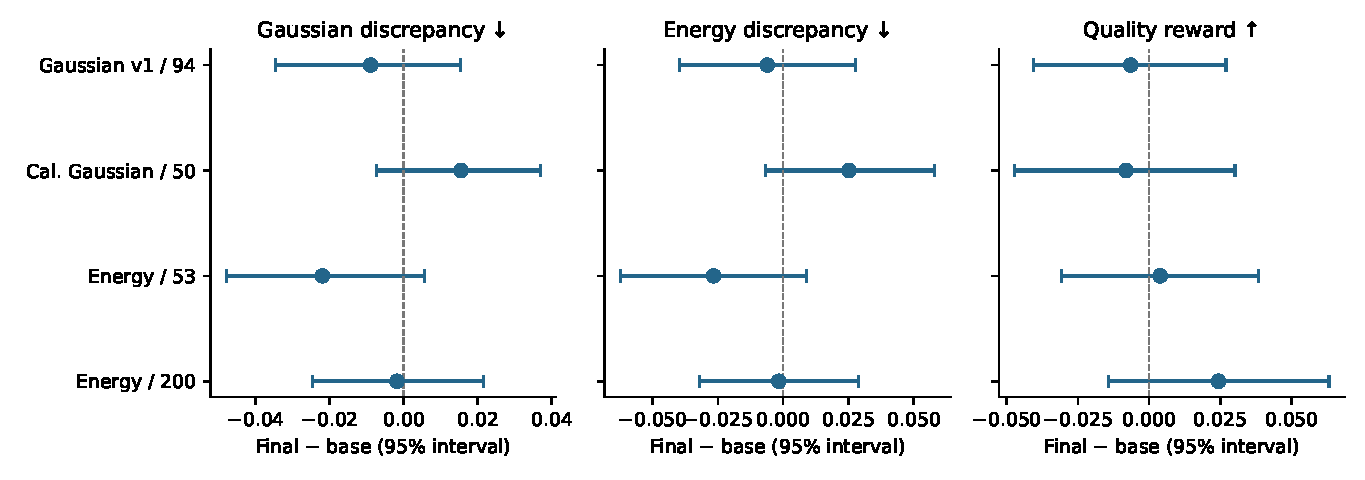
\includegraphics[width=\linewidth]{figures/semantic-changes.pdf}
 \caption{Paired question-level changes from the shared instruction baseline.
 Whiskers are exploratory bootstrap intervals (Table~\ref{tab:semantic-ci-new});
 every interval crosses zero. The 53- and 200-update energy points belong
 to one training trajectory.}
 \label{fig:semanticchanges}
\end{figure}
\begin{figure}[htbp]
 \centering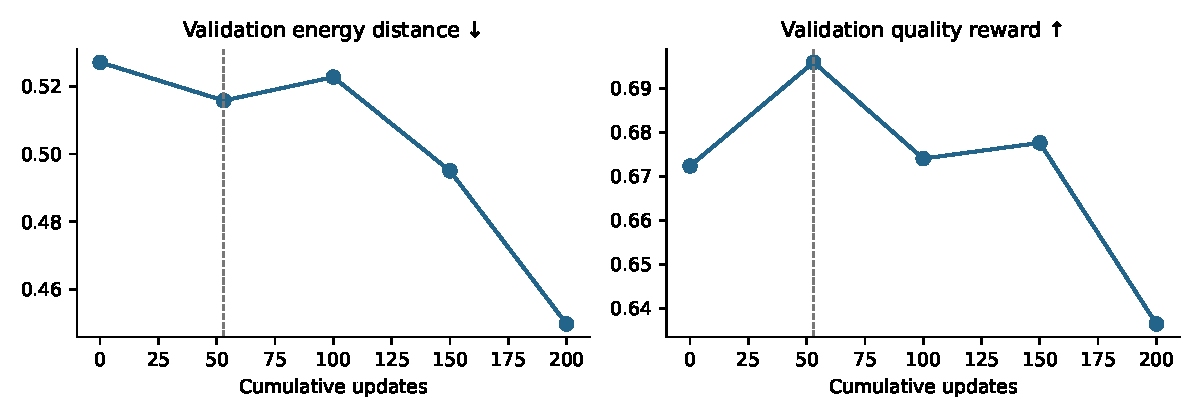
\includegraphics[width=\linewidth]{figures/energy-validation.pdf}
 \caption{Energy-run validation probes: ten questions, four answers each.
 The dashed line marks the update-53 checkpoint resumed by the continuation.
 These validation values use different questions from the final test and
 must not be compared as the same curve. Lines join saved probes only;
 they do not imply monotonic training progress.}
 \label{fig:energyvalidation}
\end{figure}
\FloatBarrier

\subsection{Four-question distribution-only fitting diagnostic}
To isolate limited in-sample fitting, a fresh base actor is trained on
four fixed eligible training questions, with 16 independent answers per
question per update (64 globally). Eligibility requires a single-turn
5--100-word prompt, both references 80--350 words, and reference-length
ratio at most two. Sorted eligible IDs are selected with seed 42;
four unseen original-validation questions are selected with seed 43.
The original 19-question test set is unused in this diagnostic.

Quality credit is exactly zero, with no reward scorer or quality judge
loaded. The retained objective is
\begin{equation}
 \mathcal L_{\mathrm{diag}}=
 \frac{0.5s_E\,\E_c D_E(P_c^{\mathrm{ref}},Q_{\theta,c})
      +0.002\,\E_c\KL(\pi_\theta\Vert\pi_0)}{1.502}.
 \label{eq:diagnosticloss}
\end{equation}
The divisor is deliberately unchanged when quality is removed. Centered
policy KL, fixed features/references and energy scale are retained.
The new schedule uses five warmup updates and a planned 100-step cosine
decay, cut off by a 70-minute policy-stage limit. The job completes
17 updates and 1,088 answers in a scheduler time of 1h18m37s.
This is a fresh small-question fitting test, not an ablation that changes
only the quality coefficient of the prior 102-question run.

Seen evaluation uses 32 answers per question (128 total), unseen 16
(64 total), with matched RNG isolated from training.
Seen energy distance falls 0.52614 to 0.50614 (3.80\%), with three of
four questions improving; intermediate update 10 is 0.5197.
The four-question mean-change interval is $[-0.0546,0.0111]$.
Unseen distance rises 0.58786 to 0.59691 (1.54\%), with mean-change
interval $[-0.0086,0.0277]$ (Table~\ref{tab:diagnostic-new}).
The evidence supports a modest, uncertain fitting signal and no
demonstrated generalization. It neither proves that fitting is
impossible nor establishes that the quality reward caused earlier
matching difficulty. Quality was not measured here.
\begin{table}[htbp]
\centering\small
\caption{Distribution-only diagnostic: four fixed training questions (seen), 32 evaluation answers each; four validation questions (unseen), 16 each. Quality is neither rewarded nor measured.}\label{tab:diagnostic-new}
\begin{tabular}{@{}lrrrr@{}}
\toprule
Scope / policy & Gaussian & Energy & Words & EOS (\%)\\
\midrule
Seen base & 0.4447 & 0.5261 & 561.6 & 81.2\\
Seen RL & 0.4282 & 0.5061 & 561.6 & 79.7\\
Unseen base & 0.4478 & 0.5879 & 469.3 & 57.8\\
Unseen RL & 0.4543 & 0.5969 & 458.8 & 59.4\\
\bottomrule
\end{tabular}
\end{table}


\subsection{Post hoc word and character distribution audits}
The following CPU analyses reuse saved diagnostic generations without
new sampling. Each compares outputs with the same exact question's
two references and averages question metrics equally. Word targets
pool references by word counts, unlike equal-answer weighting of the
semantic prototypes. All words enter numerical metrics; display-only
stopword filtering does not alter them. Forward KL uses total generated
pseudocount mass one. JSD and total variation are unsmoothed, with
an OTHER category for out-of-reference items.

\begin{table}[htbp]
\centering\small
\caption{Post hoc exact-question word matching on saved diagnostic outputs. Both reference answers are pooled by word count; question metrics are averaged equally. KL uses total generated pseudocount mass one; JSD and TV are unsmoothed with OTHER.}\label{tab:word-audit-new}
\begin{tabular}{@{}lrrr@{}}
\toprule
Scope / policy & Word KL & Word JSD & Word TV\\
\midrule
Seen base & 1.3325 & 0.2726 & 0.5478\\
Seen RL & 1.2785 & 0.2712 & 0.5483\\
Unseen base & 1.6379 & 0.3003 & 0.5923\\
Unseen RL & 1.6590 & 0.3005 & 0.5931\\
\bottomrule
\end{tabular}
\end{table}


Seen word KL falls by 4.05\%, but JSD changes only slightly and TV
worsens slightly. Unseen word KL, JSD and TV all worsen
(Table~\ref{tab:word-audit-new}). Matching an embedding objective does
not ensure matching lexical marginals, even with question-specific
references. These are post hoc JSD measurements, not a JSD training arm.

The character audit uses two explicit feature choices: raw
case-sensitive Unicode code points including whitespace, punctuation
and code; and lowercase English letters a--z only. References are
pooled by character count. With the same smoothing/OTHER conventions,
raw seen KL slightly worsens, while letters-only KL slightly improves
on both scopes (Table~\ref{tab:character-audit-new}). Raw unseen KL
increases from 0.18580 to 0.18955; its recorded four-question bootstrap
interval for the change is $[0.00076,0.00754]$. The other three
character-KL intervals include zero. These exploratory, post hoc
four-question summaries do not include training-seed or reference
uncertainty and are not corrected for multiple comparisons. Agreement
on common letters is particularly weak evidence for correct code,
vocabulary matching or semantic coverage.
\begin{table}[htbp]
\centering\scriptsize
\caption{CPU-only character-unigram audit of the same diagnostic samples. Each pair of columns is base $\to$ RL. Raw counts preserve case, spaces, newlines and punctuation; letters retain lowercase a--z only. Reference pooling is by character count; KL smoothing and OTHER follow the word audit.}\label{tab:character-audit-new}
\begin{tabular}{@{}lrrrrrrr@{}}
\toprule
Scope & Features & KL base & KL RL & JS base & JS RL & TV base & TV RL\\
\midrule
Seen & Raw Unicode & 0.09141 & 0.09165 & 0.02760 & 0.02781 & 0.11746 & 0.11695\\
Seen & Letters a--z & 0.01922 & 0.01877 & 0.00475 & 0.00463 & 0.07160 & 0.06916\\
Unseen & Raw Unicode & 0.18580 & 0.18955 & 0.03999 & 0.04111 & 0.16946 & 0.17085\\
Unseen & Letters a--z & 0.02560 & 0.02476 & 0.00635 & 0.00614 & 0.08031 & 0.07821\\
\bottomrule
\end{tabular}
\end{table}


\subsection{Recorded evidence and interpretation}
The text sequence contains both promising and negative results. The
Shakespeare trials improve distribution diagnostics and their shared
training judge; later HelpSteer trials do not establish a robust joint
benefit under stronger, separate model audits. Conditional reference
matching removes the conceptual mismatch of comparing unrelated questions,
but two references, frozen features and small conditional batches remain
restrictive. Calibration changes coefficient balance; centering preserves
the expected KL gradient. Neither implementation correctness nor a
reasonable objective guarantees a measurable policy improvement in the
available budget.

The source package includes the exact comparison/audit JSONs, configs,
source hashes, question-level semantic statistics, bootstrap settings,
and generated vector figures. The character audit is a local CPU record
with hashes verified against the committed diagnostic samples. All
training runs logged to the \texttt{stochastic-llm} W\&B project under
\texttt{yash2007-university-of-washington}; the included run records link
to the historical jobs. The source snapshot is repository commit
\texttt{deb5c8e} plus the recorded local character audit and manuscript
analysis. These records support reproducibility; upstream model/data
overlap, one seed, repeated diagnostic inspection and absence of new
human ratings remain material limits.
